\documentclass[../main.tex]{subfiles}
\begin{document}
\subsection{Quantitative as Categorical}

Unlike in section~\ref{sec:categorical}, some datasets have a very large number of observations or the observations are a vector of quantitative measurements that work in tandem. One approach for handling these types of datasets is to develop categorical representations of these quantitative variables.  



\subsubsection{Radial Charts}
\label{sec:radial}
One method of transforming quantitative vectors into categorical representations is to visualize the vector using a radial graph. Radial visualizations are designed to show composite indicators (CI) \cite{chambers_graphical_1983}; a CI is a type of visualization where the multivariate observation is mapped to a single visual idiom. For example, the line representing the observation vector in a parallel coordinates plot is a CI. 
\begin{figure}[H]
    \begin{subfigure}{\textwidth}
    \centering
    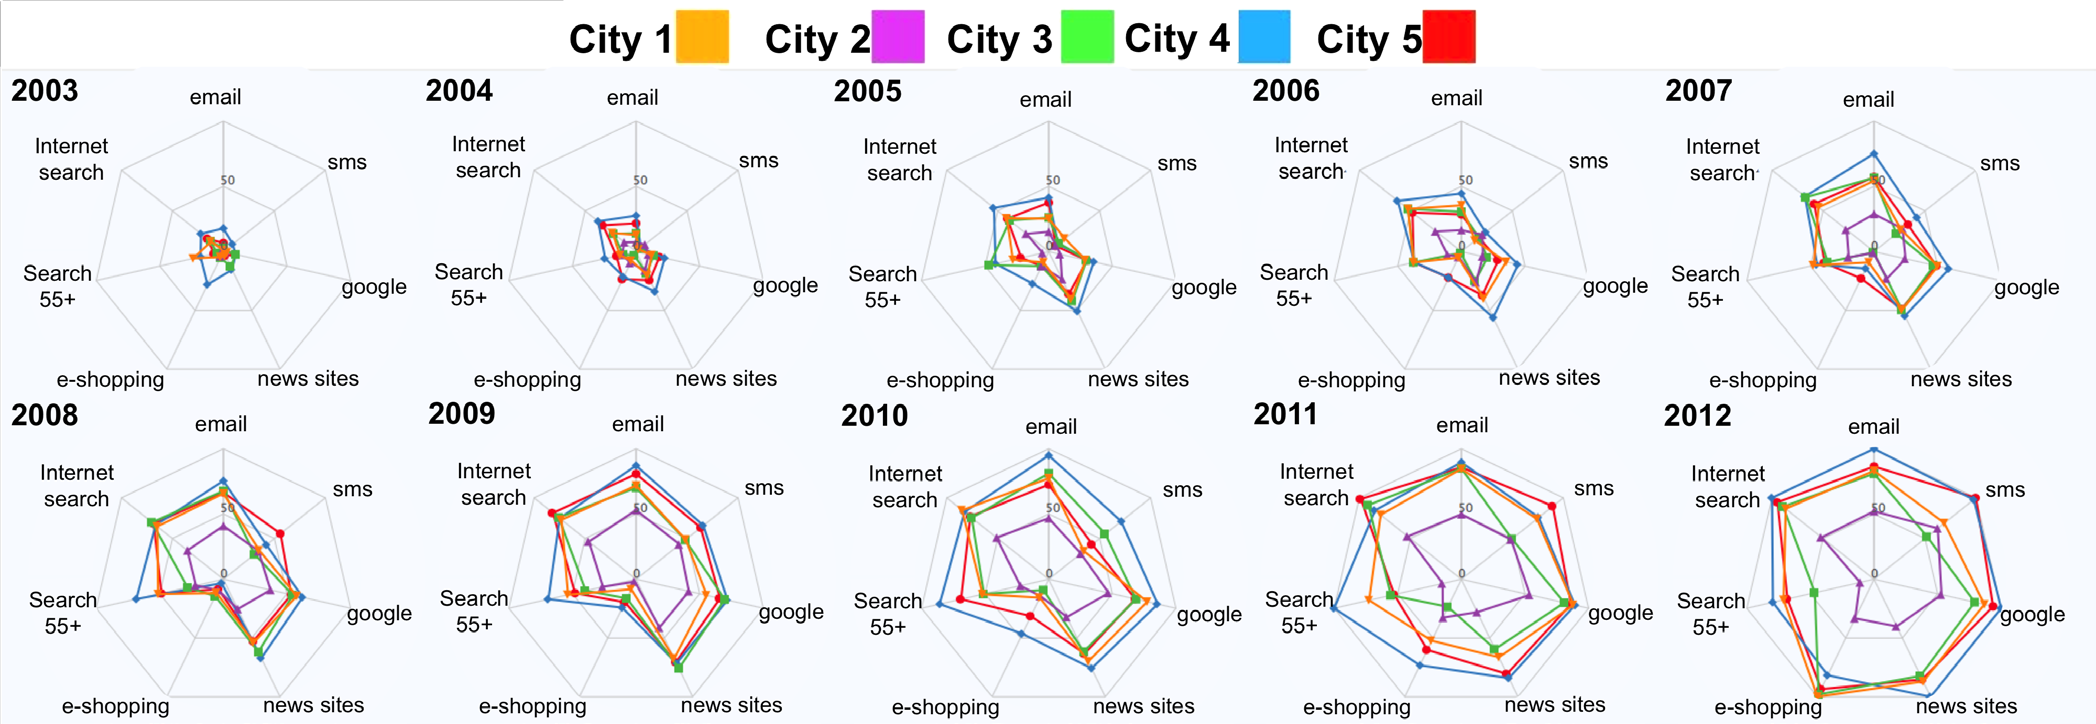
\includegraphics[scale=0.2]{cities.png}
    \caption{The size and shape of each polygon acts as an indicator of Internet usage over time.}
    \label{fig:radarchart}
    \end{subfigure}

    \bigskip
    \begin{subfigure}{\textwidth}
    \centering
    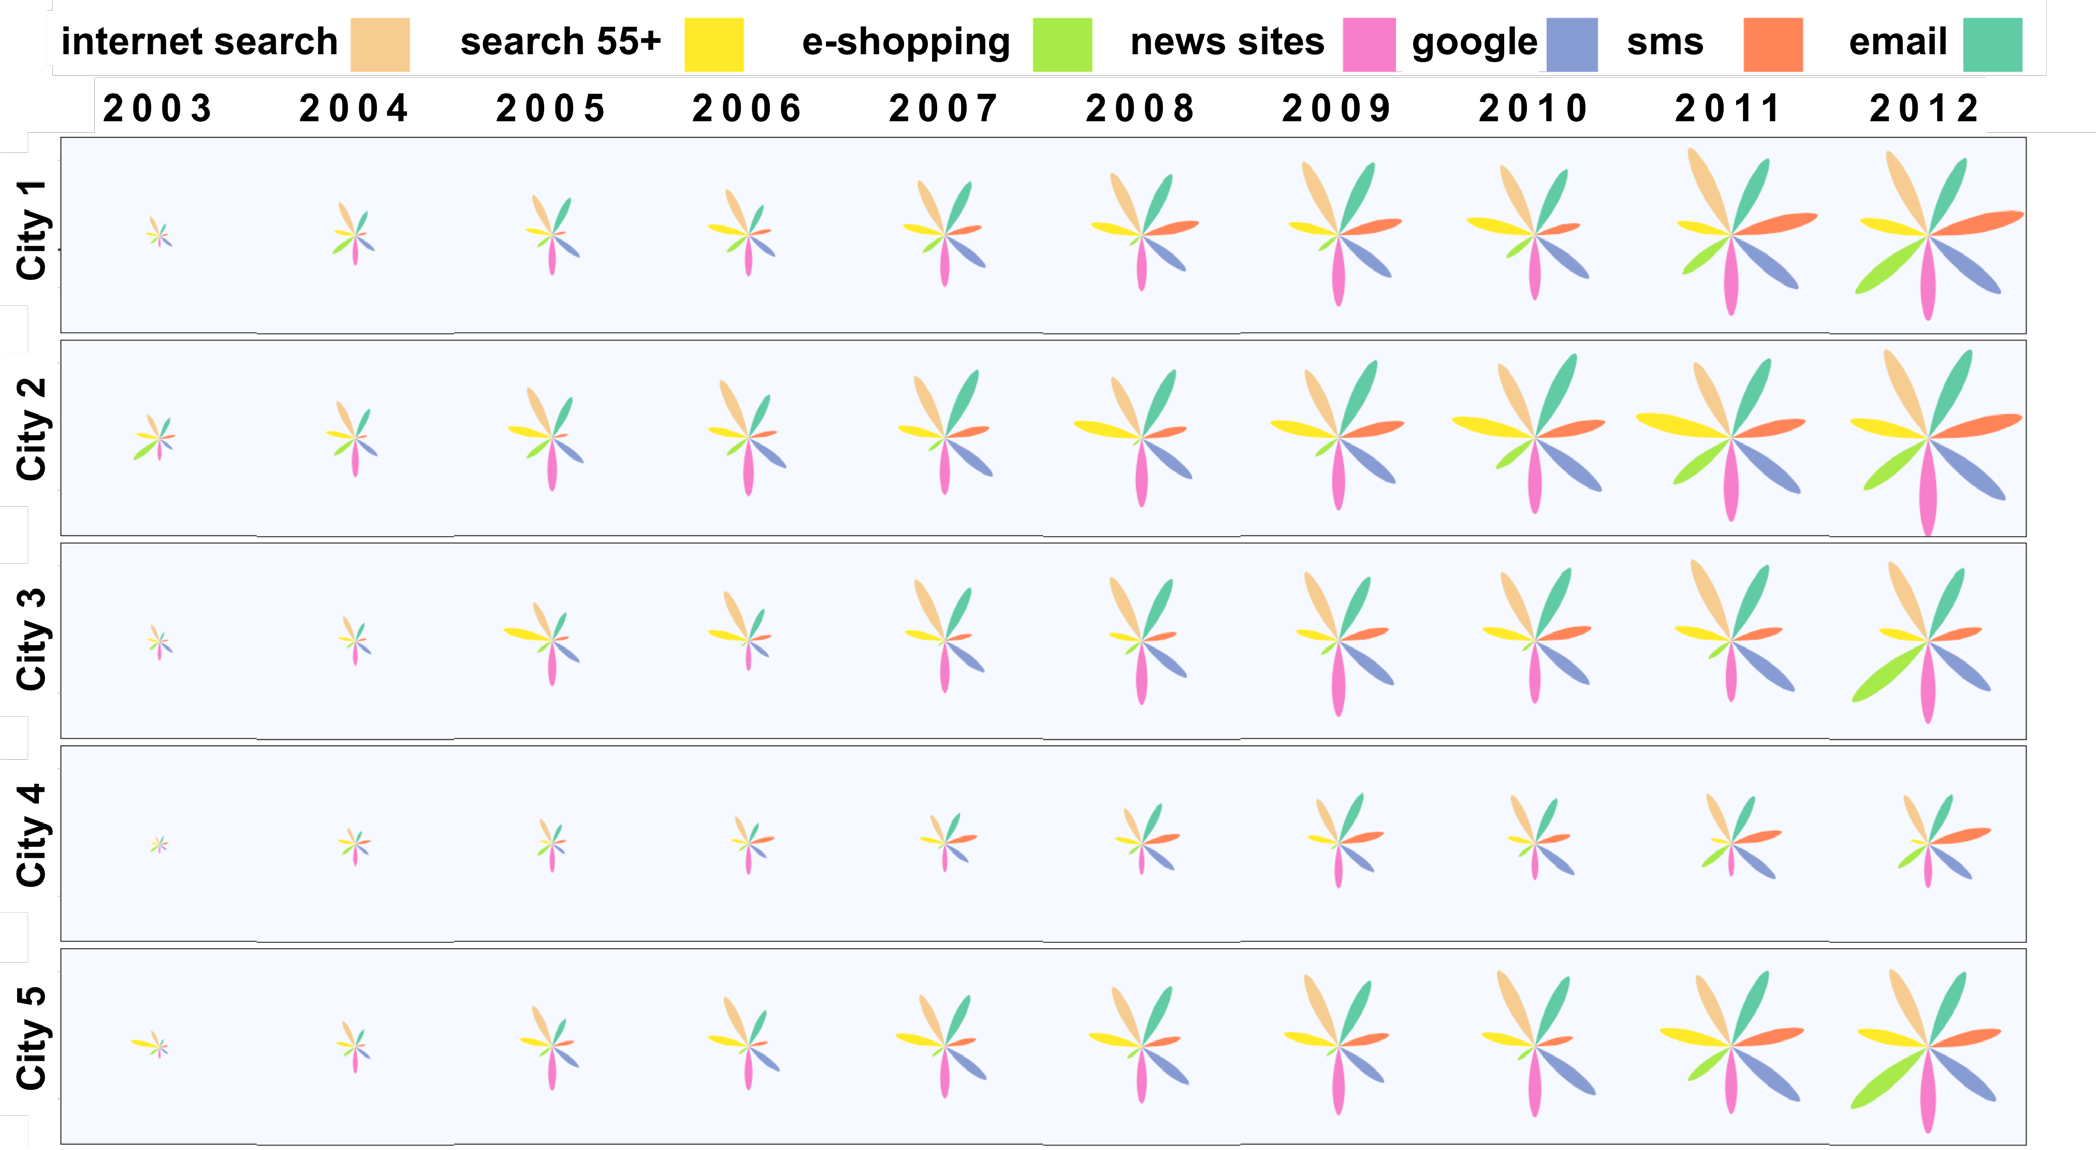
\includegraphics[scale=0.15]{flower.png}
    \caption{The size of each flower indicates Internet usage. The grid arrangement in this chart facilitates comparison both across time (horizontally) and city (vertically).}
    \label{fig:flowerchart}
    \end{subfigure}

    \bigskip
    \begin{subfigure}{\textwidth}
    \centering
    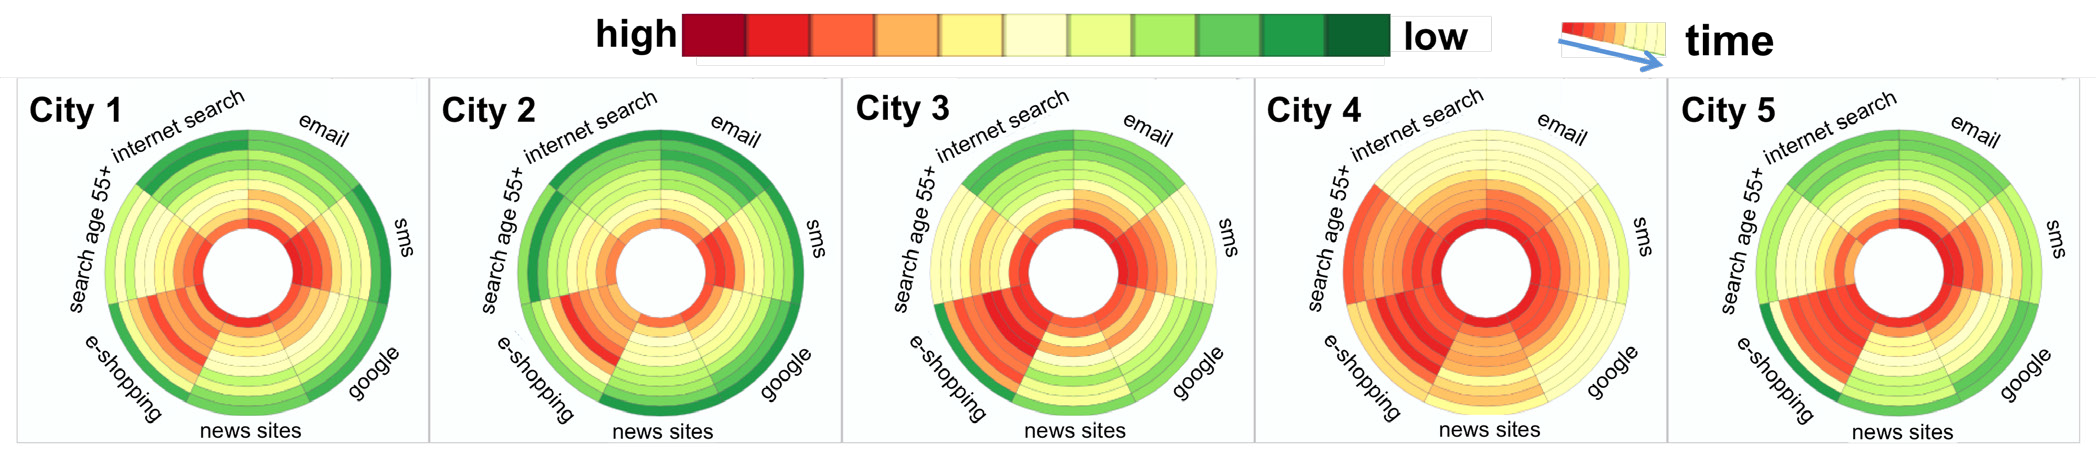
\includegraphics[width=1\linewidth]{circle.png}
    \caption{The circle chart prioritizes intensity of each type of usage, most clearly showing the popularity of shopping and SMS. This visualization facilitates testing a hypothesis of a conditional dependency amongst the Internet usage variables by isolating similar pairwise color patterns in the presence and absence of a third usage type.}
    \label{fig:circlechart}
    \end{subfigure}
\caption{Internet usage in 5 cities from 2003 to 2012. Since all types of Internet usage in all the cities seem to have expanded over time, this suggests a conditional dependence of different types of usage on time. Images are from \textit{Off the Radar: Comparative Evaluation of Radial Visualization Solutions for Composite Indicators} \cite{albo_off_2016}}
\label{fig:radial}
\end{figure}
A radar plot, as shown in figure~\ref{fig:radarchart}, is a parallel coordinate plot (PCP) where the ends of the line representing the observation are joined. Like a PCP, the radar chart shows pairwise relationships between variables that share nodes, but the radial shape also means that the polygon it forms encodes information about the relationship between all the variables. In figure~\ref{fig:radarchart} in 2010, the more rectangular shape of the city 2 Polygon relative to city 4's trapezoidal polygon signifies a characteristic difference between Internet usage in the two cities. Since figure~\ref{fig:radarchart} is arranged in small multiples of radar charts showing changes over time, by city, and across multiple types of usage, the figure can be used to examine whether this is a conditional dependency on time or city or usage type. Similarly, the flower chart in figure~\ref{fig:flowerchart} also highlights a potential dependency on time due to the flowers progressively getting larger across time. The circle chart in figure~\ref{fig:circlechart} differs from the other charts in figure~\ref{fig:radial} because time progressions are not as readily visible. Instead this chart (especially if the colormap had more steps) most clearly visualizes the frequency of the different types of Internet usage. Figure~\ref{fig:circlechart} shows that shopping and sms seem to happen in tandem, and that clear color delineation also makes it easier for a user to scan the other variables to see how frequently they occur given the relationship between shopping and SMS. The radar, flower, and circle chart visualize Internet usage as circles to varying degrees of success, but radar charts are limited to how much information can reasonably fit on one circle or a small number of circles. 


\subsubsection{Clustering}

\label{sec:cluster}
\begin{figure}[H]
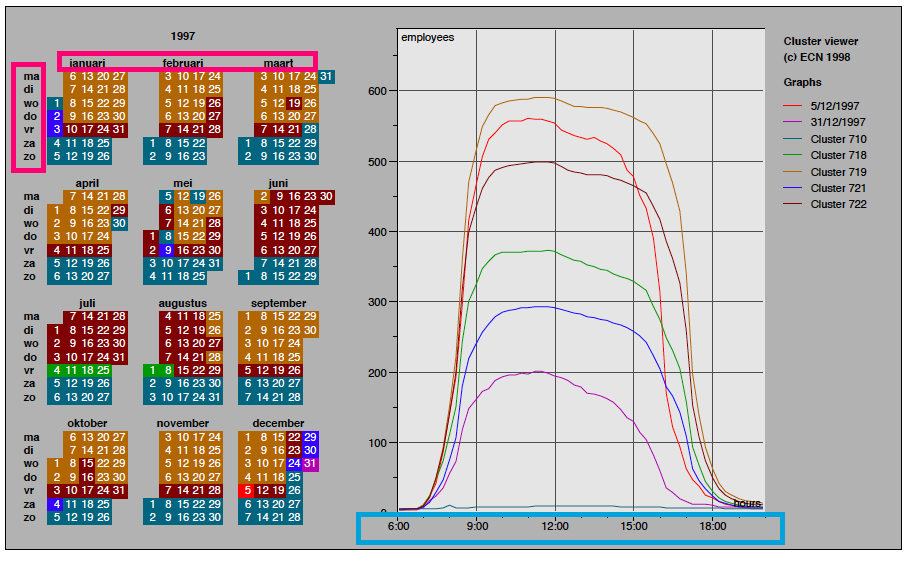
\includegraphics[width=1\textwidth]{calendar.png}
\caption{Van Wijk and Van Selow visualized the number of employees present at a research facility. This visualization shows that daily attendance seems to be more strongly dependent on the day of the week than on the time of day or the day of the year. Figure is from \textit{Cluster and Calendar based Visualization of Time Series Data} \cite{van_wijk_cluster_1999}}
\label{fig:calendar}
\end{figure}

If the data is too big for techniques that try to visualize the observations directly, one approach is to instead visualize representational fingerprints of common or outlying events in the dataset. This is frequently done through the use of a clustering algorithm. Figure~\ref{fig:calendar} shows an analysis of employee attendance at a research facility in the Netherlands \cite{van_wijk_cluster_1999}. The individual observations were recorded every 6 hours for a year, so the resulting dataset was a $(\text{day} \times \text{hours})$ matrix of the number of employees at work for that day and time. To reduce the dimensionality of this dataset to something easier to visualize, they used an agglomerative clustering algorithm \cite{kaufman_agglomerative_1990} where the days were observations and the hours were the feature vectors. The results of this clustering were used to create daily attendance curves representative of the days in each cluster; these representative curves are shown in the timeseries plot in figure~\ref{fig:calendar}. They visualized the cluster membership of the days by coloring them the same as their representative cluster, and preserved the temporal structure of the data by presenting this cluster membership as a calendar. The researchers found that both the shape and magnitude of the attendance curve changed relative to the day of the week, indicating a conditionally dependent relationship between attendance and the day of the week. While the visualization Van Wijk and Van Selow built is very specific to the question they were tackling, clustering techniques and the use of visual idioms related to the structure of the data (such as a calendar to present discretized time information) can be readily generalized. The main limitations to applying their approach to other datasets are that clustering inherently reduces dimensions and clustering techniques are limited when the dataset is a mix of categorical and quantitative variables.
\end{document}